% Copyright (c) 2014,2016 Casper Ti. Vector
% Public domain.

\chapter{区块链技术}

区块链技术作为当下作为最火热的技术之一,从09年以比特币的形式出现在人们的视野中,就一直被大家关注和讨论。本章节将从比特币出发,给出区块链技术的整体概况,其后将对区块链技术中的核心部分共识机制和智能合约进行简要介绍,最后简单列举区块链技术典型应用场景。

\section{比特币}


比特币作为一个P2P电子货币系统,是由中本聪在08年中的一篇论文中提出\cite{nakamoto2008bitcoin}的。本小节将给出比特币协议的简要概括。



\noindent\textbf{比特币网络}

比特币是构建在一个P2P网络上的数字货币系统,网络中的节点负责分发并记录交易,客户端通过与该系统的交互完成转账等操作。区块链作为比特币的核心,其被该网络中的所有节点以只追加的方式维护,并且通过工作共识机制保证每个节点上存储的内容是一致的。区块链是由一系列通过哈希值相连的区块组成的,每个区块中包含了比特币网络中被广播的交易。

比特币中的节点通过计算来确定下一区块的生产者,在确定生产者的过程中需要每个节点同时去解决一个工作量证明的问题,即所谓的挖矿,对于特定的区块$B$需要计算:

\begin{equation}\label{eqGenCmpPk}
SHA256(SHA256(B)) = (0^l||{0,1}^{256-l})
\end{equation}

其中$l$由前面产生的区块链来决定,来保证整个网络中的区块产生速度平均在每10分钟一块。当一个参与者找到一个有效的方案时,将可以去生成一个新的块,并将这个块广播给网络中的所有节点。如果该块被其它节点验证是有效的(包括块内包含交易的有效性和工作量证明的有效性等),该块将会被接受并添加到区块链上,重复以上过程来增加区块链的长度,进而完成网络中交易的记录。

比特币提供了两方面的激励来促使节点去挖取新的块,第一种是当成功的挖取到一个新的块时,新块的创建者可以获得奖励,当前的奖励为12.5个比特币;第二种奖励来之交易的交易费,纳入块的交易所支付的交易费可以归块的创建者拥有。


\noindent\textbf{比特币交易}

比特币交易包含了多个输入和输出。每个输出通过一个两元组来表示$(a,V)$,其中$a$是发送比特币的数量,$V$是一个关于谁有权花掉这笔钱的声明。在比特币中,这个声明被称作$scriptPubKey$,它是由栈式非图灵完备语言书写的比特币脚本。交易的输入指向一个前面交易的输出,同时包含第二个脚本$scriptSig$,可以用于$scriptPubKey$的代码和数据。Coinbase交易不需要纳入一个先前的交易输出作为输入。

为了向Bob发送d个比特币,Alice需要Bob的ECDSA公钥$pk_b$,并将其哈希和发送的数量$d$以及一些其它的指令放置在$scriptPubKey$中作为一个交易的输出,当然,这笔交易需要至少需要$d$数量的比特币作为输入,如\ref{code:tx}所示。如果输入的金额大于输出的金额,而且交易提交者没有设置额外的转账地址的话,剩余的金额将会被作为交易费支付给将其纳入块的节点。一旦这笔交易被广播到网络中并收入到一个有效的块中,相应的比特币就属于Bob所有了。如果Bob想花掉这笔钱,他需要将这笔交易的输出作为新建交易的输入,并附带上包含$pk_b$对应私钥$pr_b$签名的$scriptSig$即可。

\begin{lstlisting}[caption={比特币交易实例}, label=code:tx]
Input:
  Previous tx: 0205937d9faaa1a313b7826fdab...
  Index: 0
  scriptSig: odc23450cdf8cdc710e5e92af7647...

Output:
  Value: 500000
  scriptPubkey: OP_DUP OP_HASH160 a45f275794fd2337ebf7ddd018c11a21fb6c283 OP_EQUALVERIFY OP_CHECKSIG

\end{lstlisting}


\noindent\textbf{匿名性}

匿名并不是比特币设计时所考虑的目标。比特币只能通过公钥和hash来提供假名,用户在使用过程中可以生成任意多的账户。事实上,很多比特币客户端在交易过程中生成新的身份来保证用户的隐私。

虽然比特币并没有将匿名性作为其设计的目标,比特币用户希望付出一定的代价来获取匿名性,比如有掉钱的风险或者支付更多的交易费用。比如通过交易混合\cite{bonneau2014mixcoin}的技术来减弱交易地址之间的关联性,使得难易追溯资金的流向;或者通过环签名或者零知识证明\cite{kosba2016hawk}的方案提供匿名性。


比特币作是一种去中心化的数字货币,该系统中不存在中心化的银行或货币发行者,其上的货币通过奖励的方式产生,并且奖励的数目会随着时间而减少。

\section{共识机制}

区块链网络中的节点需要对新生成块中的交易及顺序达成共识,从而达到相同的状态,否则任何节点都可以产生分支而导致分叉。如果网络中的节点各自拥有不同的状态,那么该网络就无法对所有操作做出相同的判断,这个系统就不能协同运行下去。在一个分布式的p2p网络中,在没有第三方协调分歧的情况下,就需要有一种机制来保证每个节点可以达到相同的状态,而区块链上的共识机制就解决这一问题的,保证网络中各个节点的一致性。

在理想的情况下,所有的验证节点对下一个区块中的交易顺序进行投票,根据大多数人的选择来确定下一区块如何产生。但是在一个公开且没有身份管控的开放网络中,任何人都可以自由的加入,将会遭受到女巫攻击\cite{douceur2002sybil}:单一节点可以拥有多个身份表示,通过控制系统中的大部分节点来左右网络向对自己有利的方向进行。也就是说,少数的个体可以通过女巫攻击完成对整个网络的控制。

比特币通过提高产生块的计算量来解决这一问题,使得在网络中添加多个实体并不能发起女巫攻击,因为对于单个实体而言,其计算资源是有限的。更具体一点,网络中的任意节点都可以去产生下一个块,但是其需要找到一个正确的随机值(nonce)填入到区块的头部,使得产生块的哈希拥有至少指定数量的前导零\cite{antonopoulos2014mastering}。任何节点都可以对这个问题进行尝试求解,也就是所谓的工作量证明(proof of work),来完成对下一区块的构建\cite{nakamoto2008bitcoin}。在该过程中使用的是单向哈希函数,当一个节点宣称自己找到一个解的时候,其它节点很容易的去验证是否符合要求,但在给出目标的时候却无法直接确定输入应该是什么,只能通过不断尝试来玩寻求答案。

依照上述方案,当网络中的节点同时计算出下一个块时,依旧有可能存在分叉的情况。但这种分叉并不会带来影响,因为比特币中的工作量证明机制规定节点应该在工作量最大的链上进行下一区块的产生,而两个分叉的区块基本上不可能同时产出下一个块,先产生块的分支将会成为网络中被网络中节点选中的链,会有更大的几率成为更长的链,这使得网络又恢复到了统一的状态。

在比特币中使用的哈希算法是SHA-256,其它的哈希算法如Blake-256和scrypt也在被使用,同时还有一些共识机制中混入多种哈希算法。

工作量证明的方式虽然简单有效,但是其需要很多计算资源才能进行区块的产生,并且大量的计算导致能源浪费。权益证明(proof-of-stake)是另外一种替代POW的共识算法,根据节点的账户余额来决定下一块的生成权;与POW相比,POS拥有自己优势和劣势,并且其应用在起来也十分的复杂。

空间和时间一直是两个对立面,很多算法为了降低时间复杂度不得不牺牲大量空间,最近另外一种名为容量证明共识机制也被很多研究者讨论。容量证明\cite{ateniese2014proofs}的原理是需要大量的空间去寻求一个谜题的答案,如果能够给出给定问题的解,那么证明其拥有住够多的空间。具体而言,容量证明会基于矿工的公钥进行初始化,这将耗费矿工大量的磁盘空间,并将初始化的相关内容存储在矿工的计算机中;其后在挖矿的过程中,需要对区块链上的谜题进行求解,每个矿工根据本地存储相关内容,通过对磁盘的扫描获得对应的解,并完成区块的生成。以上两个过程分别是初始化过程和挖矿过程,值得注意的是,初始化过程是一个很慢的过程,单个矿工可能需要耗费数天来完成初始化,这样做的目的为了防止提过快速的计算硬件来替代存储;对于挖矿过程而言,是一个极快的过程,只需要对磁盘进行扫描即可,并不需要像工作量证明那样耗费大量的能源。随着硬件的运算能力越来越高,工作量证明的方式从原有的CPU挖矿已经转变成ASIC挖矿,使用容量证明的方式可以抗ASIC挖矿,这也是广大研究者对其感兴趣的原因。


\section{智能合约}

智能合约的概念于1994年被Nick Szabo提出\cite{szabo1996smart},是一种旨在以信息化方式传播、验证或执行合同的计算机协议,允许在没有可信第三方的情况下进行交易,完成的交易将是可追溯且不可逆的。Szabo建议将合同的条款转换成代码,并将代码放置在特定的软件或者硬件环境中运行,减少交易方对可信中介的依赖,以及第三方的避免不端行为或者意外操作。由于一般网络中缺少可信的执行方,使得智能合约在提出之后并没有被广泛应用,而区块链提供了可信的执行环境,因此智能合约在区块链出现之后逐渐被火热起来。

在区块链的环境下,智能合约是存储在区块链上的脚本。由于智能合约存在于链上,每个智能合约会拥有独一无二的地址,并通过发起对相应地址的交易来实现对智能合约的调用。收到出发交易后,智能合约将会在每个节点上按照合约的设定,自动独立地执行合约内容。事实上在每个节点上都运行着一个虚拟机(VM)来执行合约代码,区块链网络充当着分散式VM的角色。

区块链技术最开始仅仅是用于转账交易的记录,而智能合约的应用使得在区块链上可以开发出功能更加丰富的应用。用户根据自身的需求,使用智能合约语言将需要的逻辑操作编写成合约代码,并以交易的形式发布到区块链上,该步骤即为智能合约的书写和部署。当智能合约存在于区块链上之后,用户就可以向合约的地址发送交易来调用合约,完成合约内容的执行,即智能合约的调用。


不同区块链平台合约语言的自身性质将决定智能合约能够实现的操作,如比特币上使用的基于堆栈的脚本语言,指令集小并且不支持循环等复杂运算,可以实现的功能就很有限。从以太坊之后的区块链平台,基本上都拥有图灵完备的合约语言,能够实现各种应用逻辑,极大的扩展了区块链本身的功能,可以应用在数字货币之外的场景。特别是对于金融领域、智能资产、托管支付等许多场景都能通过智能合约来实现。区块链为智能合约的执行提供了可信的环境,而智能合约则给区块链赋予了更加宽广的应用场景。



\section{区块链的应用}

区块链技术最初只是被用于比特币中完成一个数字货币的构建,但区块链技术具有去中心化和防篡改的特性而被逐渐延伸到其它应用场景。比较典型的应用包括金融、物联网、社会公共服务、名誉系统和安全和隐私5个方面\cite{zheng2016blockchain},如图\ref{fig:applications}所示。

\begin{figure}[htbp]
 	\centering
 	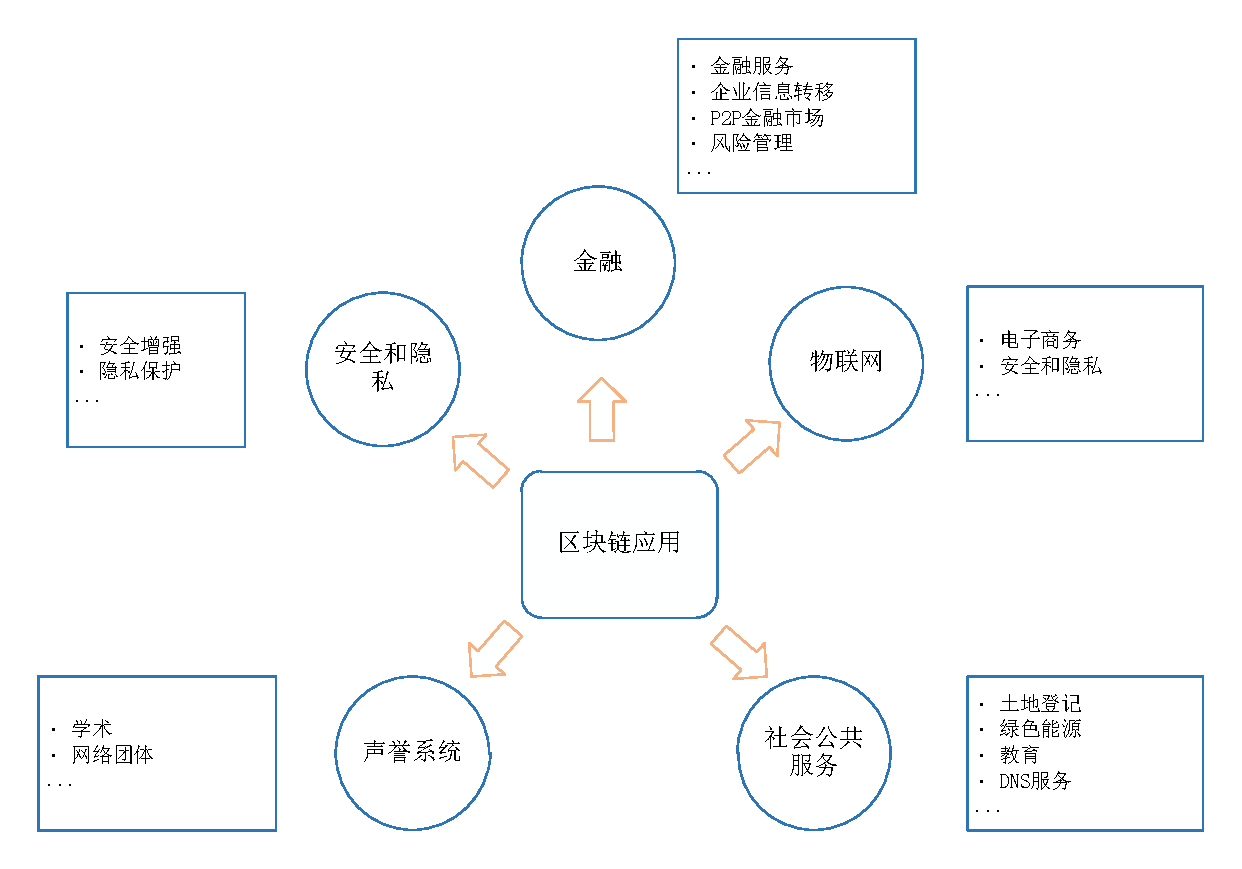
\includegraphics[width = 0.8\textwidth]{img/applications}
 	\caption{区块链典型的应用领域}\label{fig:applications}
\end{figure}

金融方面的应用包括金融服务、p2p金融市场、风险管理等,其中比特币、以太坊就是传统金融服务的另外一种表现形式,区块链给金融相关的应用带来了更好的特性;物联网方面的应用旨在使用区块链技术完成物联网实体之间数据的交换并提高自身的安全和隐私;与社会公共服务相关的区块链应用包括土地注册、绿色能源方面、教育和DNS服务等方面;名誉系统旨在利用区块链的不可篡改的特性,记录如学术论文或者网络团体的行为,提供有效的声誉证明。


% vim:ts=4:sw=4



















